% Lattice points (q,p); convergents to sqrt(2).
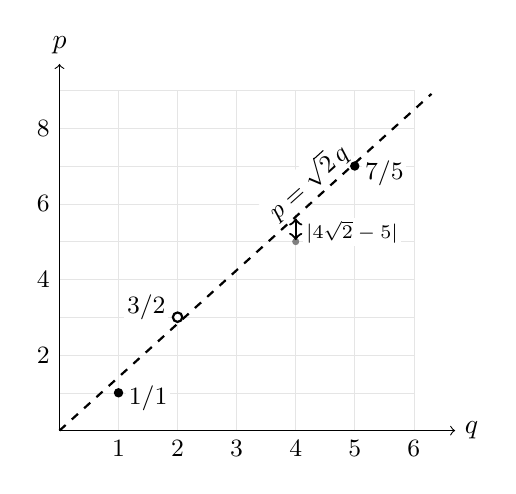
\begin{tikzpicture}[x=.75cm,y=.48cm]
\draw[step=1,gray!20,very thin] (0,0) grid (6,9);
\draw[->] (0,0)--(6.7,0) node[right] {$q$};
\draw[->] (0,0)--(0,9.7) node[above] {$p$};
\draw[thick,dashed] (0,0)--(6.3,8.9095);
\node[rotate=42,font=\small,fill=white,inner sep=1pt] at (4.2,6.6) {$p=\sqrt2\,q$};
\foreach \x in {1,...,6} {\node[below,font=\small] at (\x,0) {\x};}
\foreach \y in {2,4,6,8} {\node[left,font=\small] at (0,\y) {\y};}
\fill (1,1) circle[x radius=.08,y radius=.125];
\fill (5,7) circle[x radius=.08,y radius=.125];
\draw[thick,fill=white] (2,3) circle[x radius=.08,y radius=.125];
\node[right,font=\small,fill=white,inner sep=1pt] at (1.12,.85) {$1/1$};
\node[left,font=\small,fill=white,inner sep=1pt] at (1.85,3.25) {$3/2$};
\node[right,font=\small,fill=white,inner sep=1pt] at (5.12,6.8) {$7/5$};
\fill[gray] (4,5) circle[x radius=.06,y radius=.094];
\draw[<->,thick] (4,5.04)--(4,5.61685);
\node[right,font=\scriptsize,fill=white,inner sep=1pt] at (4.12,5.25) {$|4\sqrt2-5|$};
\end{tikzpicture}
